% Options for packages loaded elsewhere
\PassOptionsToPackage{unicode}{hyperref}
\PassOptionsToPackage{hyphens}{url}
%
\documentclass[
  openany]{book}
\usepackage{amsmath,amssymb}
\usepackage{lmodern}
\usepackage{iftex}
\ifPDFTeX
  \usepackage[T1]{fontenc}
  \usepackage[utf8]{inputenc}
  \usepackage{textcomp} % provide euro and other symbols
\else % if luatex or xetex
  \usepackage{unicode-math}
  \defaultfontfeatures{Scale=MatchLowercase}
  \defaultfontfeatures[\rmfamily]{Ligatures=TeX,Scale=1}
\fi
% Use upquote if available, for straight quotes in verbatim environments
\IfFileExists{upquote.sty}{\usepackage{upquote}}{}
\IfFileExists{microtype.sty}{% use microtype if available
  \usepackage[]{microtype}
  \UseMicrotypeSet[protrusion]{basicmath} % disable protrusion for tt fonts
}{}
\makeatletter
\@ifundefined{KOMAClassName}{% if non-KOMA class
  \IfFileExists{parskip.sty}{%
    \usepackage{parskip}
  }{% else
    \setlength{\parindent}{0pt}
    \setlength{\parskip}{6pt plus 2pt minus 1pt}}
}{% if KOMA class
  \KOMAoptions{parskip=half}}
\makeatother
\usepackage{xcolor}
\IfFileExists{xurl.sty}{\usepackage{xurl}}{} % add URL line breaks if available
\IfFileExists{bookmark.sty}{\usepackage{bookmark}}{\usepackage{hyperref}}
\hypersetup{
  pdftitle={D I F F R N A : A RNA-Seq analysis pipeline},
  pdfauthor={Izem Mouhoubi; Théo Roncalli; Gustavo Magaña López},
  hidelinks,
  pdfcreator={LaTeX via pandoc}}
\urlstyle{same} % disable monospaced font for URLs
\usepackage{color}
\usepackage{fancyvrb}
\newcommand{\VerbBar}{|}
\newcommand{\VERB}{\Verb[commandchars=\\\{\}]}
\DefineVerbatimEnvironment{Highlighting}{Verbatim}{commandchars=\\\{\}}
% Add ',fontsize=\small' for more characters per line
\usepackage{framed}
\definecolor{shadecolor}{RGB}{248,248,248}
\newenvironment{Shaded}{\begin{snugshade}}{\end{snugshade}}
\newcommand{\AlertTok}[1]{\textcolor[rgb]{0.94,0.16,0.16}{#1}}
\newcommand{\AnnotationTok}[1]{\textcolor[rgb]{0.56,0.35,0.01}{\textbf{\textit{#1}}}}
\newcommand{\AttributeTok}[1]{\textcolor[rgb]{0.77,0.63,0.00}{#1}}
\newcommand{\BaseNTok}[1]{\textcolor[rgb]{0.00,0.00,0.81}{#1}}
\newcommand{\BuiltInTok}[1]{#1}
\newcommand{\CharTok}[1]{\textcolor[rgb]{0.31,0.60,0.02}{#1}}
\newcommand{\CommentTok}[1]{\textcolor[rgb]{0.56,0.35,0.01}{\textit{#1}}}
\newcommand{\CommentVarTok}[1]{\textcolor[rgb]{0.56,0.35,0.01}{\textbf{\textit{#1}}}}
\newcommand{\ConstantTok}[1]{\textcolor[rgb]{0.00,0.00,0.00}{#1}}
\newcommand{\ControlFlowTok}[1]{\textcolor[rgb]{0.13,0.29,0.53}{\textbf{#1}}}
\newcommand{\DataTypeTok}[1]{\textcolor[rgb]{0.13,0.29,0.53}{#1}}
\newcommand{\DecValTok}[1]{\textcolor[rgb]{0.00,0.00,0.81}{#1}}
\newcommand{\DocumentationTok}[1]{\textcolor[rgb]{0.56,0.35,0.01}{\textbf{\textit{#1}}}}
\newcommand{\ErrorTok}[1]{\textcolor[rgb]{0.64,0.00,0.00}{\textbf{#1}}}
\newcommand{\ExtensionTok}[1]{#1}
\newcommand{\FloatTok}[1]{\textcolor[rgb]{0.00,0.00,0.81}{#1}}
\newcommand{\FunctionTok}[1]{\textcolor[rgb]{0.00,0.00,0.00}{#1}}
\newcommand{\ImportTok}[1]{#1}
\newcommand{\InformationTok}[1]{\textcolor[rgb]{0.56,0.35,0.01}{\textbf{\textit{#1}}}}
\newcommand{\KeywordTok}[1]{\textcolor[rgb]{0.13,0.29,0.53}{\textbf{#1}}}
\newcommand{\NormalTok}[1]{#1}
\newcommand{\OperatorTok}[1]{\textcolor[rgb]{0.81,0.36,0.00}{\textbf{#1}}}
\newcommand{\OtherTok}[1]{\textcolor[rgb]{0.56,0.35,0.01}{#1}}
\newcommand{\PreprocessorTok}[1]{\textcolor[rgb]{0.56,0.35,0.01}{\textit{#1}}}
\newcommand{\RegionMarkerTok}[1]{#1}
\newcommand{\SpecialCharTok}[1]{\textcolor[rgb]{0.00,0.00,0.00}{#1}}
\newcommand{\SpecialStringTok}[1]{\textcolor[rgb]{0.31,0.60,0.02}{#1}}
\newcommand{\StringTok}[1]{\textcolor[rgb]{0.31,0.60,0.02}{#1}}
\newcommand{\VariableTok}[1]{\textcolor[rgb]{0.00,0.00,0.00}{#1}}
\newcommand{\VerbatimStringTok}[1]{\textcolor[rgb]{0.31,0.60,0.02}{#1}}
\newcommand{\WarningTok}[1]{\textcolor[rgb]{0.56,0.35,0.01}{\textbf{\textit{#1}}}}
\usepackage{longtable,booktabs,array}
\usepackage{calc} % for calculating minipage widths
% Correct order of tables after \paragraph or \subparagraph
\usepackage{etoolbox}
\makeatletter
\patchcmd\longtable{\par}{\if@noskipsec\mbox{}\fi\par}{}{}
\makeatother
% Allow footnotes in longtable head/foot
\IfFileExists{footnotehyper.sty}{\usepackage{footnotehyper}}{\usepackage{footnote}}
\makesavenoteenv{longtable}
\usepackage{graphicx}
\makeatletter
\def\maxwidth{\ifdim\Gin@nat@width>\linewidth\linewidth\else\Gin@nat@width\fi}
\def\maxheight{\ifdim\Gin@nat@height>\textheight\textheight\else\Gin@nat@height\fi}
\makeatother
% Scale images if necessary, so that they will not overflow the page
% margins by default, and it is still possible to overwrite the defaults
% using explicit options in \includegraphics[width, height, ...]{}
\setkeys{Gin}{width=\maxwidth,height=\maxheight,keepaspectratio}
% Set default figure placement to htbp
\makeatletter
\def\fps@figure{htbp}
\makeatother
\setlength{\emergencystretch}{3em} % prevent overfull lines
\providecommand{\tightlist}{%
  \setlength{\itemsep}{0pt}\setlength{\parskip}{0pt}}
\setcounter{secnumdepth}{5}
\usepackage{booktabs}
\usepackage{amsthm}
\makeatletter
\def\thm@space@setup{%
  \thm@preskip=8pt plus 2pt minus 4pt
  \thm@postskip=\thm@preskip
}
\makeatother
\ifLuaTeX
  \usepackage{selnolig}  % disable illegal ligatures
\fi
\usepackage[]{natbib}
\bibliographystyle{apalike}

\title{D I F F R N A : A RNA-Seq analysis pipeline}
\author{Izem Mouhoubi \and Théo Roncalli \and Gustavo Magaña López}
\date{2021-11-29}

\begin{document}
\maketitle

{
\setcounter{tocdepth}{1}
\tableofcontents
}
\hypertarget{prerequisites}{%
\chapter{Prerequisites}\label{prerequisites}}

\hypertarget{hardware-and-operating-system}{%
\section{Hardware and Operating System}\label{hardware-and-operating-system}}

The pipeline was developed and tested on \href{https://fridge.ubuntu.com/2021/08/27/ubuntu-20-04-3-lts-released/}{Ubuntu 20.04.3 LTS}
on top of the \texttt{(GNU/Linux\ 5.4.0-88-generic\ x86\_64)} kernel. The output of the commands \texttt{uname} and \texttt{neofetch} are provided to further detail our configuration.

\begin{Shaded}
\begin{Highlighting}[]
\ExtensionTok{$}\NormalTok{ uname }\AttributeTok{{-}a}
\ExtensionTok{Linux}\NormalTok{ machine329a7396{-}059f{-}41aa{-}94c7{-}4c41b4ec8290 5.4.0{-}88{-}generic }\CommentTok{\#99{-}Ubuntu SMP Thu Sep 23 17:29:00 UTC 2021 x86\_64 x86\_64 x86\_64 GNU/Linux}

\ExtensionTok{$}\NormalTok{ neofetch}
            \ExtensionTok{.{-}/+oossssoo+/{-}.}\NormalTok{               ubuntu@machine3f9ae3dc{-}6a4d{-}46b7{-}8131{-}04f00a1be146 }
        \KeywordTok{\textasciigrave{}}\BuiltInTok{:}\NormalTok{+ssssssssssssssssss+:}\KeywordTok{\textasciigrave{}}           \AttributeTok{{-}{-}{-}{-}{-}{-}{-}{-}{-}{-}{-}{-}{-}{-}{-}{-}{-}{-}{-}{-}{-}{-}{-}{-}{-}{-}{-}{-}{-}{-}{-}{-}{-}{-}{-}{-}{-}{-}{-}{-}{-}{-}{-}{-}{-}{-}{-}{-}{-}{-}} 
      \ExtensionTok{{-}+ssssssssssssssssssyyssss+{-}}\NormalTok{         OS: Ubuntu 20.04.3 LTS x86\_64 }
    \ExtensionTok{.ossssssssssssssssssdMMMNysssso.}\NormalTok{       Host: OpenStack Compute 18.2.1{-}1.el7 }
   \ExtensionTok{/ssssssssssshdmmNNmmyNMMMMhssssss/}\NormalTok{      Kernel: 5.4.0{-}88{-}generic }
  \ExtensionTok{+ssssssssshmydMMMMMMMNddddyssssssss+}\NormalTok{     Uptime: 13 hours, 14 mins }
 \ExtensionTok{/sssssssshNMMMyhhyyyyhmNMMMNhssssssss/}\NormalTok{    Packages: 719 }\ErrorTok{(}\ExtensionTok{dpkg}\KeywordTok{)}\ExtensionTok{,}\NormalTok{ 4 }\ErrorTok{(}\ExtensionTok{snap}\KeywordTok{)} 
\ExtensionTok{.ssssssssdMMMNhsssssssssshNMMMdssssssss.}\NormalTok{   Shell: bash 5.0.17 }
\ExtensionTok{+sssshhhyNMMNyssssssssssssyNMMMysssssss+}\NormalTok{   Theme: Adwaita [GTK3] }
\ExtensionTok{ossyNMMMNyMMhsssssssssssssshmmmhssssssso}\NormalTok{   Icons: Adwaita [GTK3] }
\ExtensionTok{ossyNMMMNyMMhsssssssssssssshmmmhssssssso}\NormalTok{   Terminal: /dev/pts/0 }
\ExtensionTok{+sssshhhyNMMNyssssssssssssyNMMMysssssss+}\NormalTok{   CPU: Intel }\ErrorTok{(}\ExtensionTok{Haswell,}\NormalTok{ no TSX, IBRS}\KeywordTok{)} \KeywordTok{(}\ExtensionTok{16}\KeywordTok{)} \ExtensionTok{@}\NormalTok{ 2.294GHz }
\ExtensionTok{.ssssssssdMMMNhsssssssssshNMMMdssssssss.}\NormalTok{   GPU: 00:02.0 Cirrus Logic GD 5446 }
 \ExtensionTok{/sssssssshNMMMyhhyyyyhdNMMMNhssssssss/}\NormalTok{    Memory: 635MiB / 64323MiB }
  \ExtensionTok{+sssssssssdmydMMMMMMMMddddyssssssss+}
   \ExtensionTok{/ssssssssssshdmNNNNmyNMMMMhssssss/}                              
    \ExtensionTok{.ossssssssssssssssssdMMMNysssso.}                               
      \ExtensionTok{{-}+sssssssssssssssssyyyssss+{-}}
        \KeywordTok{\textasciigrave{}}\BuiltInTok{:}\NormalTok{+ssssssssssssssssss+:}\KeywordTok{\textasciigrave{}}
            \ExtensionTok{.{-}/+oossssoo+/{-}.}
\end{Highlighting}
\end{Shaded}

This configuration was actually a virtual machine hosted on \href{https://biosphere.france-bioinformatique.fr/catalogue/}{Biosphere's RAINBio} a cloud service maintained by the French Institue of Bioinformatics (\href{https://www.france-bioinformatique.fr/en/home/}{\emph{Institut Français de Bioinformatique}}).

\hypertarget{biopipes-a-biosphere-commons-app}{%
\section{BioPipes: a Biosphere-commons app}\label{biopipes-a-biosphere-commons-app}}

The instance of the virtual machine we used is called \href{https://biosphere.france-bioinformatique.fr/catalogue/appliance/119/}{\emph{BioPipes}}. It provides the most notable bioinformatics pipeline tools:

\begin{itemize}
\tightlist
\item
  \href{https://www.nextflow.io/}{nextflow}
\item
  \href{https://snakemake.github.io/}{snakemake}
\item
  \href{https://www.commonwl.org/}{cwltool}
\end{itemize}

\hypertarget{main-tools}{%
\section{Main Tools}\label{main-tools}}

Their versions are specified to maximise reproducibility:

\begin{Shaded}
\begin{Highlighting}[]
\ExtensionTok{$}\NormalTok{ conda }\AttributeTok{{-}{-}version}
\ExtensionTok{conda}\NormalTok{ 4.11.0}
\ExtensionTok{$}\NormalTok{ nextflow }\AttributeTok{{-}v}
\ExtensionTok{nextflow}\NormalTok{ version 21.10.0.5640}
\ExtensionTok{$}\NormalTok{ docker }\AttributeTok{{-}{-}version}
\ExtensionTok{Docker}\NormalTok{ version 20.10.11, build dea9396}
\end{Highlighting}
\end{Shaded}

Detailed information about our development docker installation :

\begin{Shaded}
\begin{Highlighting}[]
\ExtensionTok{$}\NormalTok{ docker info}
\ExtensionTok{Server:}
 \ExtensionTok{Containers:}\NormalTok{ 0}
  \ExtensionTok{Running:}\NormalTok{ 0}
  \ExtensionTok{Paused:}\NormalTok{ 0}
  \ExtensionTok{Stopped:}\NormalTok{ 0}
 \ExtensionTok{Images:}\NormalTok{ 4}
 \ExtensionTok{Server}\NormalTok{ Version: 20.10.11}
 \ExtensionTok{Storage}\NormalTok{ Driver: overlay2}
  \ExtensionTok{Backing}\NormalTok{ Filesystem: xfs}
  \ExtensionTok{Supports}\NormalTok{ d\_type: true}
  \ExtensionTok{Native}\NormalTok{ Overlay Diff: true}
  \ExtensionTok{userxattr:}\NormalTok{ false}
 \ExtensionTok{Logging}\NormalTok{ Driver: json{-}file}
 \ExtensionTok{Cgroup}\NormalTok{ Driver: cgroupfs}
 \ExtensionTok{Cgroup}\NormalTok{ Version: 1}
 \ExtensionTok{Plugins:}
  \ExtensionTok{Volume:}\NormalTok{ local}
  \ExtensionTok{Network:}\NormalTok{ bridge host ipvlan macvlan null overlay}
  \ExtensionTok{Log:}\NormalTok{ awslogs fluentd gcplogs gelf journald json{-}file local logentries splunk syslog}
 \ExtensionTok{Swarm:}\NormalTok{ inactive}
 \ExtensionTok{Runtimes:}\NormalTok{ io.containerd.runc.v2 io.containerd.runtime.v1.linux runc}
 \ExtensionTok{Default}\NormalTok{ Runtime: runc}
 \ExtensionTok{Init}\NormalTok{ Binary: docker{-}init}
 \ExtensionTok{containerd}\NormalTok{ version: 7b11cfaabd73bb80907dd23182b9347b4245eb5d}
 \ExtensionTok{runc}\NormalTok{ version: v1.0.2{-}0{-}g52b36a2}
 \ExtensionTok{init}\NormalTok{ version: de40ad0}
 \ExtensionTok{Security}\NormalTok{ Options:}
  \ExtensionTok{apparmor}
  \ExtensionTok{seccomp}
   \ExtensionTok{Profile:}\NormalTok{ default}
 \ExtensionTok{Kernel}\NormalTok{ Version: 5.4.0{-}88{-}generic}
 \ExtensionTok{Operating}\NormalTok{ System: Ubuntu 20.04.3 LTS}
 \ExtensionTok{OSType:}\NormalTok{ linux}
 \ExtensionTok{Architecture:}\NormalTok{ x86\_64}
 \ExtensionTok{CPUs:}\NormalTok{ 16}
 \ExtensionTok{Total}\NormalTok{ Memory: 62.82GiB}
 \ExtensionTok{Name:}\NormalTok{ machine3f9ae3dc{-}6a4d{-}46b7{-}8131{-}04f00a1be146}
 \ExtensionTok{ID:}\NormalTok{ XT4Y:2HUL:HXEA:CDXV:ERC7:Z7JZ:YYRU:WZBT:ERCU:6GGA:OBZ6:QLXE}
 \ExtensionTok{Docker}\NormalTok{ Root Dir: /mnt/docker{-}data}
 \ExtensionTok{Debug}\NormalTok{ Mode: false}
 \ExtensionTok{Registry:}\NormalTok{ https://index.docker.io/v1/}
 \ExtensionTok{Labels:}
 \ExtensionTok{Experimental:}\NormalTok{ false}
 \ExtensionTok{Insecure}\NormalTok{ Registries:}
  \ExtensionTok{127.0.0.0/8}
 \ExtensionTok{Live}\NormalTok{ Restore Enabled: false}
\end{Highlighting}
\end{Shaded}

\hypertarget{dependencies}{%
\chapter{Dependencies}\label{dependencies}}

\hypertarget{software}{%
\section{Software}\label{software}}

The pipeline runs on \href{https://www.nextflow.io/}{nextflow} a domain-specific language created to automate data-analysis pipelines whilst maximising reproducibility.
Nextflow enables scientists to focus on their analyses, isolating different parts of the pipeline into processes whose dependencies can be dealt with using containers and virtual environments with technologies such as \href{https://www.docker.com/}{Docker}, \href{https://singularity.hpcng.org/}{Singularity}, and \href{https://www.anaconda.com/products/individual}{Anaconda}.

The recommended way to install \texttt{nextflow} is via \texttt{conda}, using \href{https://github.com/bio-TAGI/Hackathon/blob/main/nextflow_conda_env.yml}{the environment file}.

\begin{Shaded}
\begin{Highlighting}[]
\ExtensionTok{conda}\NormalTok{ env create }\AttributeTok{{-}f}\NormalTok{ nextflow\_conda\_env.yml }\CommentTok{\# will create an env called "nextflow"}
\ExtensionTok{conda}\NormalTok{ activate nextflow}
\CommentTok{\# You can edit the file at your choice, specially if the environment name conflicts}
\CommentTok{\# with a preexisting conda env on your system}
\end{Highlighting}
\end{Shaded}

Docker should be installed as well:

\begin{Shaded}
\begin{Highlighting}[]
\FunctionTok{sudo}\NormalTok{ apt install docker}
\end{Highlighting}
\end{Shaded}

Once nextflow is installed, it will automatically retrieve the docker images used within the pipeline.

\hypertarget{workflow}{%
\chapter{Workflow}\label{workflow}}

Nextflow workflows should form a \emph{DAG} (i.e.~directed acyclic graph), which represents the flow of data through the different steps
required to produce the final result.

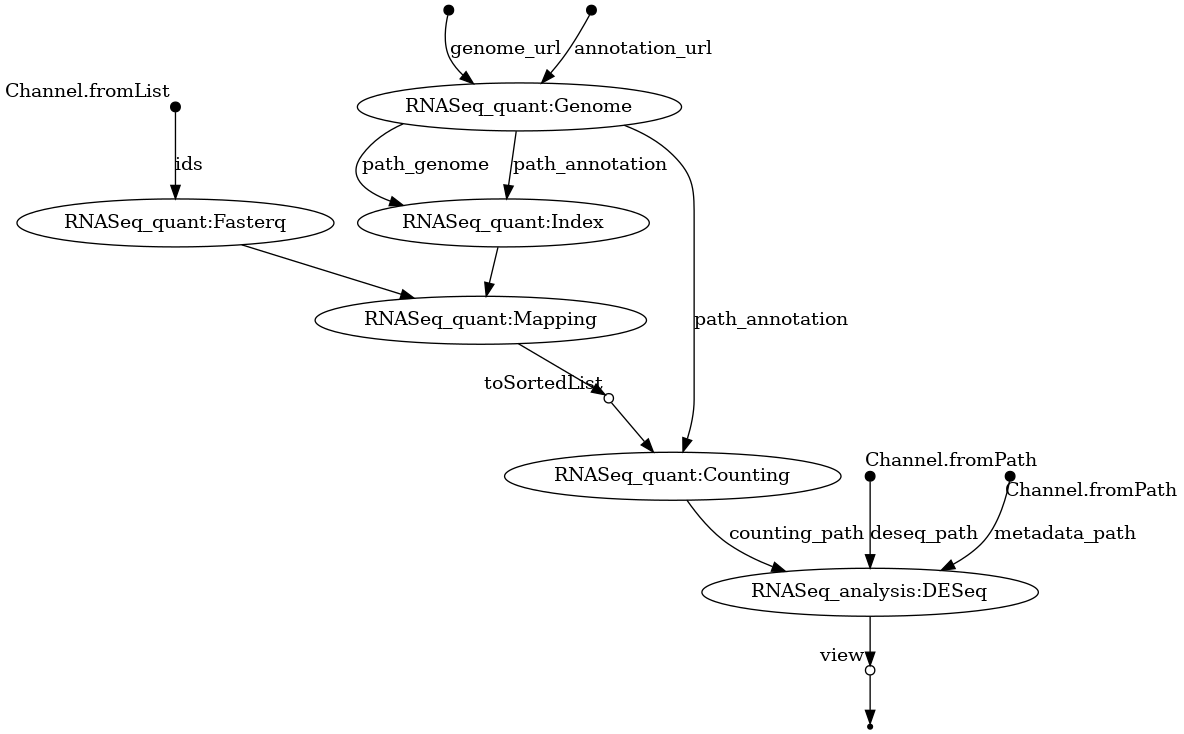
\includegraphics{images/dag.png}

This pipeline will generate a set of figures, representing differential gene expression analysis of RNA-Seq data.

\hypertarget{execution}{%
\chapter{Execution}\label{execution}}

\begin{enumerate}
\def\labelenumi{\arabic{enumi}.}
\tightlist
\item
  Clone the repo to your machine
\end{enumerate}

\begin{Shaded}
\begin{Highlighting}[]
\FunctionTok{git}\NormalTok{ clone https://github.com/bio{-}TAGI/Hackathon.git}
\BuiltInTok{cd}\NormalTok{ Hackathon}
\end{Highlighting}
\end{Shaded}

\begin{enumerate}
\def\labelenumi{\arabic{enumi}.}
\setcounter{enumi}{1}
\tightlist
\item
  Create and activate the virtual environment
\end{enumerate}

\begin{Shaded}
\begin{Highlighting}[]
\ExtensionTok{conda}\NormalTok{ env create }\AttributeTok{{-}f}\NormalTok{ nextflow\_conda\_env.yml}
\ExtensionTok{conda}\NormalTok{ activate nextflow}
\end{Highlighting}
\end{Shaded}

\begin{enumerate}
\def\labelenumi{\arabic{enumi}.}
\setcounter{enumi}{2}
\tightlist
\item
  Run the wokflow with default parameters.
\end{enumerate}

\begin{Shaded}
\begin{Highlighting}[]
\BuiltInTok{cd}\NormalTok{ Nextflow}
\ExtensionTok{nextflow}\NormalTok{ run main.nf}
\end{Highlighting}
\end{Shaded}

\begin{enumerate}
\def\labelenumi{\arabic{enumi}.}
\setcounter{enumi}{3}
\tightlist
\item
  If you had to stop the workflow run, or if some error occurred, you can always resume the execution as follows:
\end{enumerate}

\begin{Shaded}
\begin{Highlighting}[]
\ExtensionTok{nextflow}\NormalTok{ run main.nf }\AttributeTok{{-}resume}
\end{Highlighting}
\end{Shaded}

\begin{enumerate}
\def\labelenumi{\arabic{enumi}.}
\setcounter{enumi}{4}
\tightlist
\item
  Specifying parameters from the command line
\end{enumerate}

\begin{Shaded}
\begin{Highlighting}[]
\ExtensionTok{nextflow}\NormalTok{ run main.nf }\AttributeTok{{-}{-}param1}\NormalTok{ value1}\DataTypeTok{\textbackslash{}}
\NormalTok{{-}{-}param2 value2}\DataTypeTok{\textbackslash{}}
\NormalTok{{-}{-}paramn valuen }\CommentTok{\# these are generic names, not actual parameters for the pipeline}
\end{Highlighting}
\end{Shaded}

\hypertarget{parameters}{%
\chapter{Parameters}\label{parameters}}

\begin{itemize}
\tightlist
\item
  \texttt{index\_cpus} (number of cpus reserved for the genome indexation process. \texttt{default=14})
\item
  \texttt{mapping\_cpus} (idem. for the mapping process, used to create BAM files. \texttt{default=14})
\item
  \texttt{counting\_cpus} (idem. for the counting process. \texttt{default=7})
\item
  \texttt{mapping\_memory} (RAM reserved for mapping. \texttt{default=50GB})
\end{itemize}

If you already possess some of the files needed to execute the pipeline, you can specify them as follows:

\begin{itemize}
\tightlist
\item
  \texttt{reads} (path pointing to a directory containing the \texttt{fasterq} files)
\item
  \texttt{genome} (path pointing to a directory containing the genome FASTA file)
\item
  \texttt{index} (Répertoire contenant les fichiers d'index)
\item
  \texttt{mapping} (Répertoire contenant les fichiers BAM)
\item
  \texttt{counting} (Chemin d'accès entier au fichier de comptage -- comprend le fichier lui-même)
\item
  \texttt{metadata} (Chemin d'accès entier au fichier de métadonnées -- comprend le fichier lui-même)
\end{itemize}

If unspecified, the pipeline will be executed using default values from the config file : \href{https://github.com/bio-TAGI/Hackathon/blob/main/Nextflow/nextflow.config}{nextflow.config}. These too, can be tweaked and overriden:

\begin{itemize}
\tightlist
\item
  \texttt{ids} List of SRR accession number to fetch paired-end fastq files.

  \begin{itemize}
  \tightlist
  \item
    default=\texttt{{[}\textquotesingle{}SRR628582\textquotesingle{},\ \textquotesingle{}SRR628583\textquotesingle{},\ \textquotesingle{}SRR628584\textquotesingle{},\ \textquotesingle{}SRR628585\textquotesingle{},\ \textquotesingle{}SRR628586\textquotesingle{},\ \textquotesingle{}SRR628587\textquotesingle{},\ \textquotesingle{}SRR628588\textquotesingle{},\ \textquotesingle{}SRR628589\textquotesingle{}{]}}
  \end{itemize}
\item
  \texttt{genome\_url} URL to download the reference genome.

  \begin{itemize}
  \tightlist
  \item
    default \texttt{ftp://ftp.ensembl.org/pub/release-101/fasta/homo\_sapiens/dna/Homo\_sapiens.GRCh38.dna.primary\_assembly.fa.gz}
  \end{itemize}
\item
  \texttt{annotation\_url} URL to donwload the reference genome's annotation.

  \begin{itemize}
  \tightlist
  \item
    default \texttt{ftp://ftp.ensembl.org/pub/release-101/gtf/homo\_sapiens/Homo\_sapiens.GRCh38.101.chr.gtf.gz}
  \end{itemize}
\item
  \texttt{sjdbOverhang} (a STAR-specific parameter. \texttt{default=99})

  \begin{itemize}
  \tightlist
  \item
    For further information about this parameter, see \href{https://sydney-informatics-hub.github.io/training-RNAseq/02-BuildAGenomeIndex/index.html}{this tutorial},
    or the \href{https://physiology.med.cornell.edu/faculty/skrabanek/lab/angsd/lecture_notes/STARmanual.pdf}{STAR manual}.
  \end{itemize}
\end{itemize}

\hypertarget{caveats}{%
\chapter{Caveats}\label{caveats}}

\begin{itemize}
\tightlist
\item
  A good internet connection is required. Retrieving \texttt{fastq} can be really slow and is thus a bottleneck.
\item
  \href{https://github.com/ncbi/sra-tools/wiki}{\texttt{fasterq-dump}} will randomly segfault.
  At first we thought this was caused by connection problems, but running \texttt{ping} ruled this out. Apparently, the segfault is \href{https://github.com/ncbi/sra-tools/issues/518}{a known issue}.
\item
  The workflow will inevitably fail if you try building the genome's index on a machine with less than \textasciitilde30 GB of RAM available.

  \begin{itemize}
  \tightlist
  \item
    As a general rule, tweak all parameters to reasonable values that fit your setup and needs. We don't know your hardware, you do ;)
  \end{itemize}
\end{itemize}

  \bibliography{book.bib,packages.bib}

\end{document}
